\begin{figure}
  \centering
    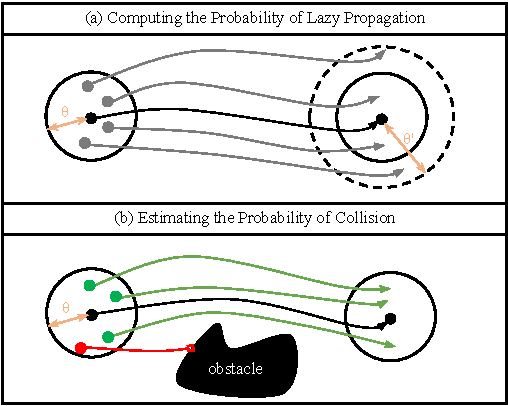
\includegraphics[width=\columnwidth,height=0.8\columnwidth]{assets/pert_mod.pdf}
  \caption{Perturbing the start state of an edge $e_i \in \mathcal{E}$ (black arrow) by a maximum of $\theta$ and applying $e_i.u$ for duration $e_i.\Delta t$ results in a perturbed end state ($\hat{q}_f$). Applying multiple random perturbations for $e_i$ (grey arrows in (a), green and red arrows in (b)) allows us to estimate $e_i.P_{\text{lazy\_prop}} = Pr(\|\hat{q}_f - e_i.q_f\|_2 < \theta) = 2/4$ and $e_i.P_{\text{collision}} = 1/4$ for the provided example. We repeat this process for all edges in $\mathcal{E}$ to integrate lazy approaches to simulation and collision checking in \textsl{LazyBoE}.}\label{fig:pert_analysis}
\end{figure}